\documentclass{beamer}
\usepackage{graphicx}
\usepackage{graphics}
\usepackage{hyperref}
\usepackage[english]{babel}
\usepackage[T1]{fontenc}
\usepackage[utf8]{inputenc}
\usepackage{xfrac}
\usepackage{array}


\mode<presentation>
{
    \usetheme{AMUFree-kk}
    \setbeamercovered{transparent = 28}
}
\title{LM again?}
\date{2021}
\author{Karol Kaczmarek}
\setbeamertemplate{bibliography item}{[\theenumiv]}


\begin{document}

\begin{frame}
    \titlepage
\end{frame}

\iffalse
\AtBeginSection[]
{
    \begin{frame}
        \frametitle{Outline}
        \tableofcontents[currentsection]
    \end{frame}
}
\fi



% Shortformer
\section{Shortformer}
\begin{frame}
    \frametitle{Shortformer \cite{shortformer}}
    \begin{itemize}
        \item 31 December 2020, University of Washington - code available (fairseq fork)
        \item \textbf{generative Transformer} (decoder) -- 16 layers of dimension 1024 with 16 heads, 4096 dimension of feedforward sublayers and 3072 sequence length
        \item \textbf{Staged Training} -- initially training on shorter subsequences
        \item \textbf{Position-Infused Attention} (PIA) -- cached representations from the previously subsequence
        \item tested on \textbf{WikiText-103}
    \end{itemize}
\end{frame}

\begin{frame}
    \frametitle{Language Model Inference}
    \begin{itemize}
        \item Training with 9216 tokens (\textbf{sequence length} x \textbf{batch size})
        \item Inference batch size of 1 (for all tests!)
    \end{itemize}
    \begin{center}
        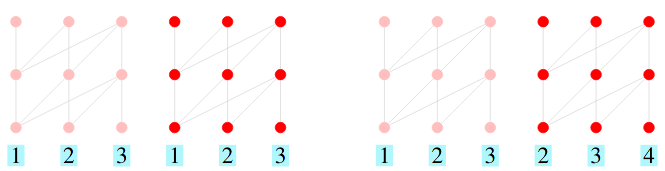
\includegraphics[scale=0.25]{img/shortformer_window.png}
        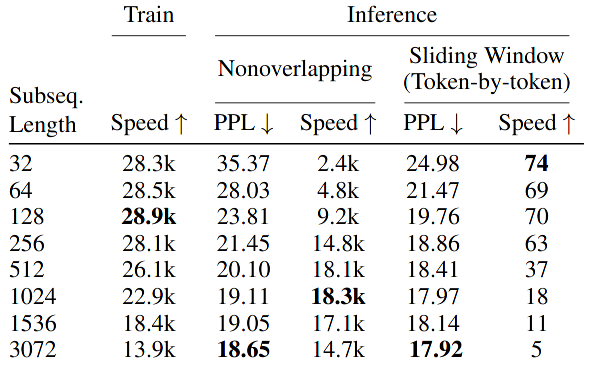
\includegraphics[scale=0.30]{img/shortformer_window_performance.png}
    \end{center}
\end{frame}

\begin{frame}
    \frametitle{Staged Training}
    \begin{itemize}
        \item \textbf{two-stage training} routine that initially uses short input subsequences followed by long subsequences (in the second use 3072 tokens)
        \item \textbf{sinusoidal position embeddings}, learned position embeddings would create a dependency between the parameterization and the subsequence length
        \item \textbf{neither modify nor reset the state of the optimization} algorithm between the two stages
    \end{itemize}
\end{frame}

\begin{frame}
    \frametitle{Staged Training -- results on dev set (205 epochs)}
    \begin{center}
        \begin{tabular}{ l l }
        \small{only 37\% of baseline time}
        & \small{1.1 perplexity better in 87\% time} \\
        \\
        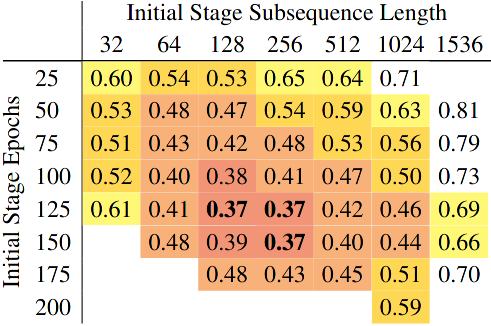
\includegraphics[scale=0.30]{img/shortformer_staged_train_time.png}
        & 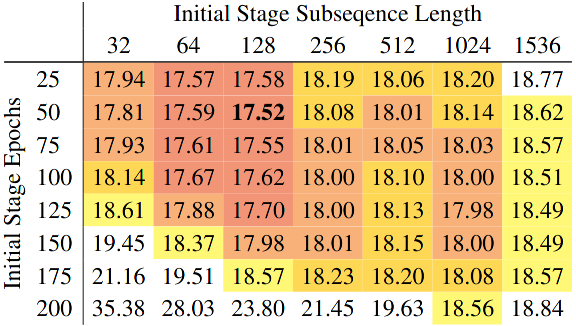
\includegraphics[scale=0.30]{img/shortformer_staged_train_perplexity.png} \\
        \scriptsize{Time until match the baseline} & \scriptsize{Perplexity at the end of training -- base line 18,65 }
        \end{tabular}
    \end{center}
    \begin{center}
        using more than two stages (up to six), did not outperform
    \end{center}
\end{frame}

\begin{frame}
    \frametitle{Repositioning Position Embeddings}
    \begin{itemize}
        \item inspired by \textbf{slide window evaluation} (very slow evaluation) and \textbf{relative position embeddings} (slow inference by 22\% and require 26\% more parameters)
        \item \textbf{Position-Infused Attention (PIA)} - reuse previous outputs by making each output contain \textbf{no positional information}:
        \begin{itemize}
           \item without using extra parameters, memory, or run time
           \item can use much shorter input subsequences and still achieve performance
        \end{itemize}
    \end{itemize}
\end{frame}

\begin{frame}
    \frametitle{Position-Infused Attention (PIA) - positional embeddings}
    \begin{center}
        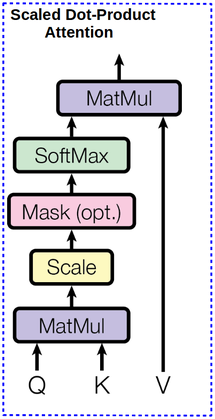
\includegraphics[scale=0.30]{img/attention.png}
        \begin{itemize}
            \item do not add position embeddings at \textbf{the beginning}, but rather adds position embeddings to \textbf{the Query} and \textbf{Key} vectors at each layer (but \textbf{not to the Value})
            \item outputs at each layer are weighted sums of \textbf{the value vectors without positional information} (value vectors do not contain positional information)
        \end{itemize}
    \end{center}
\end{frame}

\begin{frame}
    \frametitle{Position-Infused Attention (PIA) - visualization}
    \begin{center}
        \begin{tabular}{ l l }
        \scriptsize{1. Embed tokens: $ X $} & \scriptsize{1. Embed tokens: $ X $}
        \\
        \scriptsize{2. Add positional embeddings: $ X = X + P $} & \scriptsize{2. Do not add position embeddings}
        \\
        \multicolumn{2}{c}{\scriptsize{3. Feed transformer layer where self-attention:}}
        \\
        \scriptsize{ Key=$X$, Query=$X$, Value=$X$ } & \scriptsize{ Key=$X + P$, Query=$X + P$, Value=$X$ }
        \\
        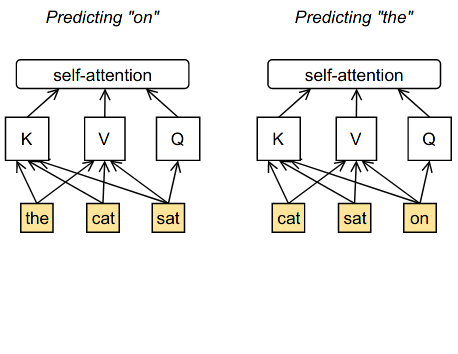
\includegraphics[scale=0.30]{img/shortformer_attention_base.png}
        & 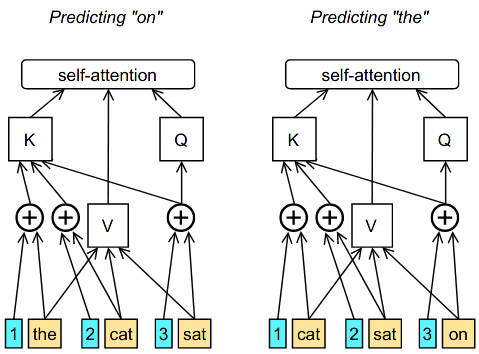
\includegraphics[scale=0.30]{img/shortformer_attention_cached.png} \\
        \end{tabular}
    \end{center}
    \begin{center}
        \scriptsize{$X$ - embedded tokens, $P$ - position embedding}
    \end{center}
\end{frame}

\begin{frame}
    \frametitle{Visualization of evaluation/training}
    \begin{center}
        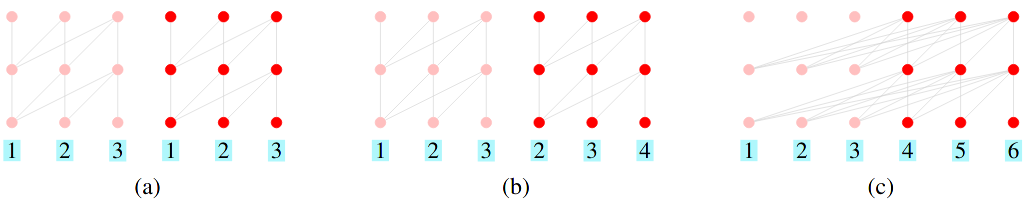
\includegraphics[scale=0.30]{img/shortformer_window_with_cache.png}
    \end{center}
    \begin{itemize}
        \item (a) - nonoverlapping training and inference
        \item (b) - sliding window inference with stride S = 1
        \item (c) - caching (In the next iteration tokens 4, 5 and 6 become the cache, and are \textbf{given position embeddings 1, 2 and 3}, while the three new tokens \textbf{get position embeddings 4, 5, and 6})
    \end{itemize}
\end{frame}

\begin{frame}
    \frametitle{Position-Infused Attention (PIA) with cache - score}
    \begin{center}
        \begin{itemize}
            \item \textbf{baseline} achieves \textbf{18.65} on the development set
            \item only PIA method (size as baseline) achieves 19.35 perplexity (speed and memory usage do not change)
            \item using PIA and caching (cached equal to \textbf{Subseq. Length}):
        \end{itemize}
        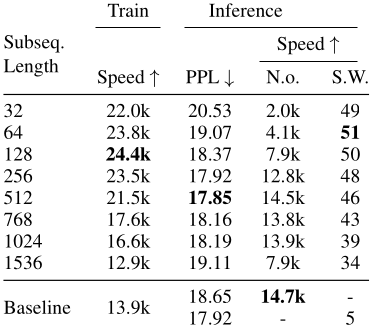
\includegraphics[scale=0.36]{img/shortformer_pia_score.png}

        \tiny{\textbf{N.o.} is Nonoverlapping, \textbf{S.W.} is Sliding Window, batch size of 1 for inference, best model trains
55\% faster}
    \end{center}
\end{frame}

\begin{frame}
    \frametitle{PIA with Staged Training - score}
    \begin{center}
        \begin{itemize}
            \item using \textbf{Position-Infused Attention} and \textbf{Staged Training} on the previous best model (PIA model with 512 tokens)
            \item the best model (\textbf{Shortformer}) achieves 17.47 perplexity and trains 65\% faster than the baseline model (18.65 perplexity)  on the development set
        \end{itemize}

        \begin{tabular}{ m{4cm} m{5cm} }
        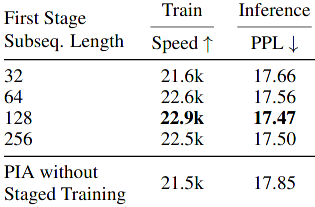
\includegraphics[scale=0.30]{img/shortformer_pia_score_with_staged_train.png}
        & 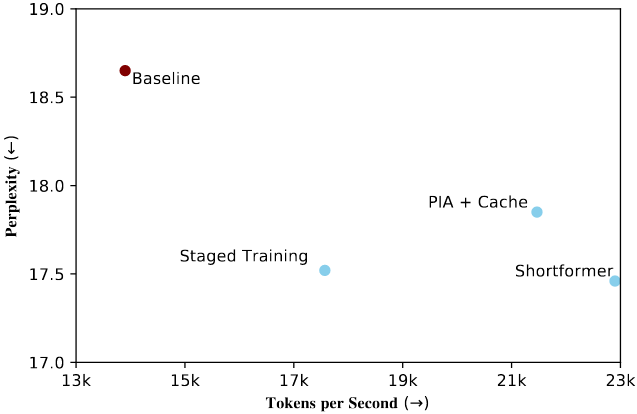
\includegraphics[scale=0.25]{img/shortformer_performance.png} \\
        \end{tabular}
    \end{center}
\end{frame}

\begin{frame}
    \frametitle{Compare to the other LMs}
    \begin{center}
        \begin{itemize}
            \item evaluate on the test set of WikiText-103
            \item \textbf{Shortformer} is almost twice as fast to train and is nine times faster in token-by-token generation
            \item sliding window evaluation cannot be used in \textbf{Shortformer} because \textbf{caching} and \textbf{PIA} were used
        \end{itemize}

        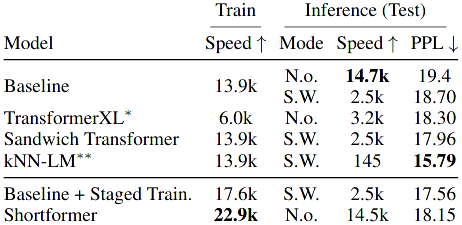
\includegraphics[scale=0.44]{img/shortformer_compare_with_other_models.png}

        \tiny{*runs on an older version of PyTorch than all other models, which might impact speed}

        \tiny{**requires a 400GB datastore}
    \end{center}
\end{frame}



% MoE
\section{Sparsely-Gated Mixture-of-Experts}
\begin{frame}
    \frametitle{Sparsely-Gated Mixture-of-Experts (MoE) \cite{moe_layer}}
    \begin{itemize}
        \item January 2017, Google + Jagiellonian University
        \item \textbf{Sparsely-Gated Mixture-of-Experts layer} (MoE) consisting of up to thousands of feed-forward sub-networks
        \item trainable \textbf{gating network} determines a sparse combination of these experts to use for each example
        \item achive greater than \textbf{1000x} improvements in model capacity with only minor losses in computational efficiency on modern GPU clusters
        \item apply the MoE to the tasks of \textbf{language modeling} and \textbf{machine translation}
    \end{itemize}
\end{frame}

\begin{frame}
    \frametitle{Mixture of Experts (MoE) layer between stacked LSTM layers}
    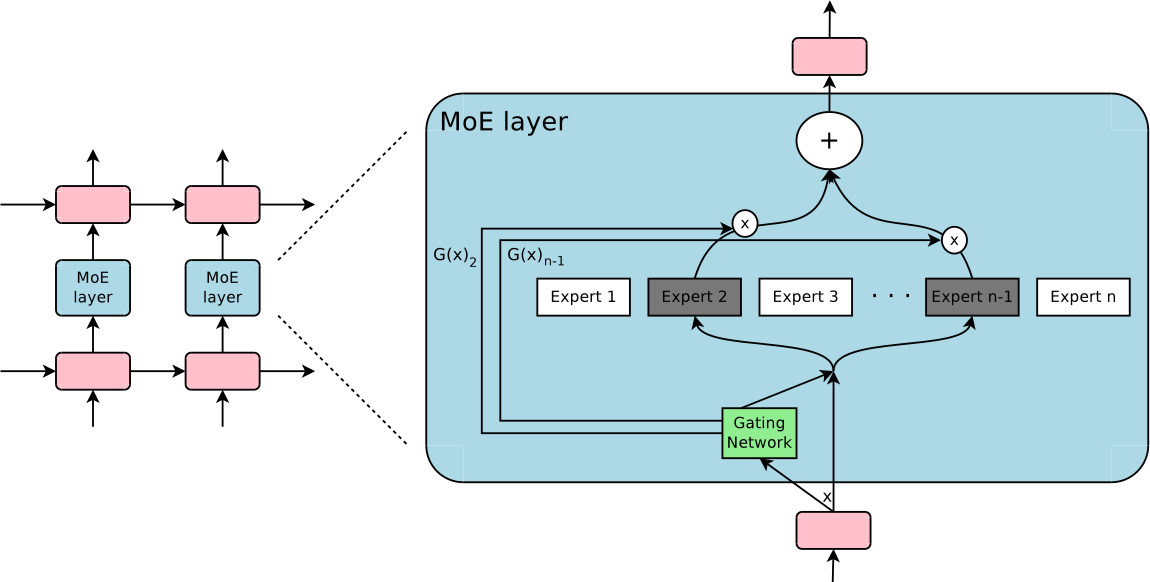
\includegraphics[scale=0.25]{img/moe_layer.png}
    \begin{itemize}
        \item \textbf{sparse gating} function selects \textbf{two experts} to perform computations
        \item outputs are \textbf{modulated} by the outputs of the \textbf{gating network}
    \end{itemize}
\end{frame}



% GShard
\section{GShard}
\begin{frame}
    \frametitle{GShard \cite{gshard}}
    \begin{itemize}
        \item June/July 2020, Google - pseudocode
        \item parallel computation patterns with \textbf{minimal changes} to the existing model code
GShard enabled us to scale up multilingual neural machine translation Transformer
model with Sparsely-Gated Mixture-of-Experts beyond \textbf{600 billion parameters}
using automatic sharding
        \item train 600B model on 2048 TPU v3 accelerators in 4 days to achieve far superior quality for translation from 100 languages to English
        \item even train 1 trillion model (\textbf{problem with stability training}, did not include the results)
    \end{itemize}
\end{frame}

\begin{frame}
    \frametitle{Sparsely-Gated Mixture-of-Experts Transformer (MoE Transformer)}
    \begin{center}
        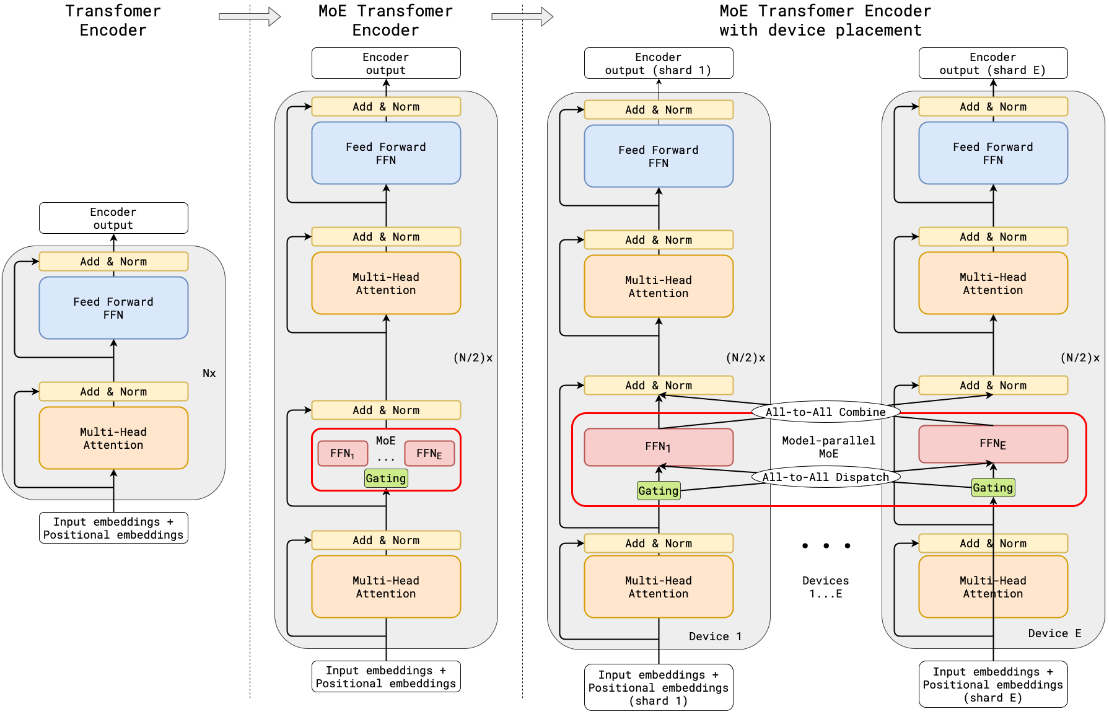
\includegraphics[scale=0.25]{img/gshard_architecture.png}
    \end{center}
\end{frame}

\begin{frame}
    \frametitle{Transformer model}
    \begin{itemize}
        \item Encoder-Decoder transformer
        \item replace every \textbf{Position-Wise Feed-Forward} layer with a \textbf{Position-wise Mixture of Experts} (MoE) layer
        \item \textbf{Position-wise Mixture-of-Experts} (MoE) layer - based on MoE \cite{moe_layer} with variations in the sparse gating function and feed-forward network with ReLU activation
        \item MoE layer consists of $E$ feed-forward network FFN$_{1}$ ... FNN$_{E}$ (recommended on expert per device)
    \end{itemize}
\end{frame}

\begin{frame}
    \frametitle{Position-wise Mixture-of-Experts Layer}
    \begin{center}
    $ G_{s,E} = $ GATE $(x_{s})$

    FFN$_{e}(x_{s})$ = $wo_{e} \cdot $ ReLU $(wi_{e} \cdot x_{s})$

    $y_{s} = \sum^{E}_{e=1} G_{s,e} \cdot $ FFN$_{e}(x_{s})$

    \tiny{$x_{s} $ - input token to the MoE layer, $w_{i}, w{o}$ - projection matrices in FFN (an expert)}
    \end{center}
    \begin{itemize}
        \item \footnotesize{$G_{s,E}$ - computed by a \textbf{gating network}, has one non-negative for each expert, most of which are zeros (token is not dispatched), token is dispatched to a very small number of experts (at most two experts). Representing how much an expert contributes to the network output.}
        \item \footnotesize{Every expert FFN$_{e}$ applies to $x_{s}$ a \textbf{fully-connected 2-layer} network using \textbf{ReLU activation} function.}
        \item \footnotesize{Output of the MoE layer, $y_{s}$, is \textbf{the weighted} average of outputs from all the selected experts.}
        \item \footnotesize{Gating function GATE($\cdot$) is modeled by a softmax activation function.}
    \end{itemize}
\end{frame}

\begin{frame}
    \frametitle{Massively Multilingual, Massive Machine Translation (M4) - score}
    \begin{center}
        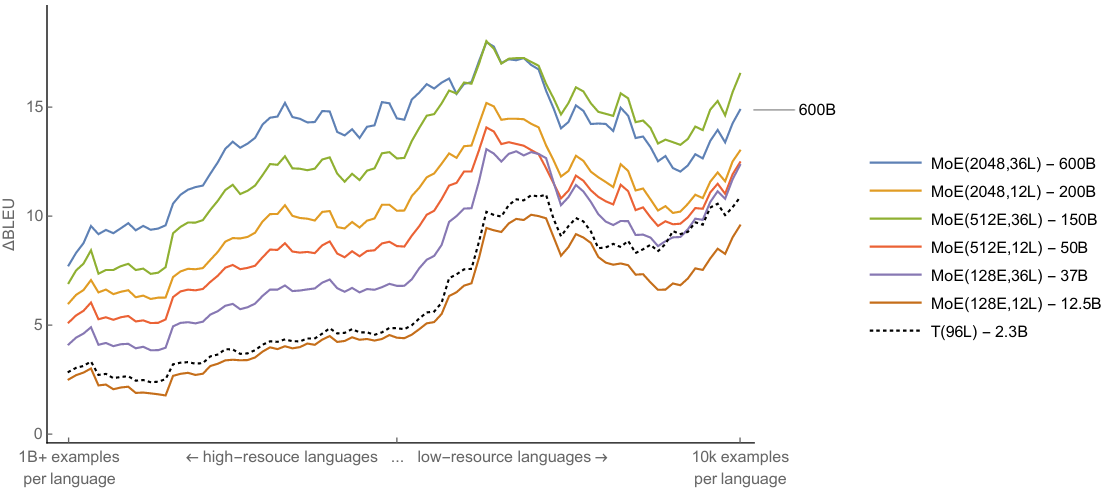
\includegraphics[scale=0.3]{img/gshard_diagram.png}
    \end{center}
\end{frame}

\begin{frame}
    \frametitle{M4 - score}
    \begin{center}
        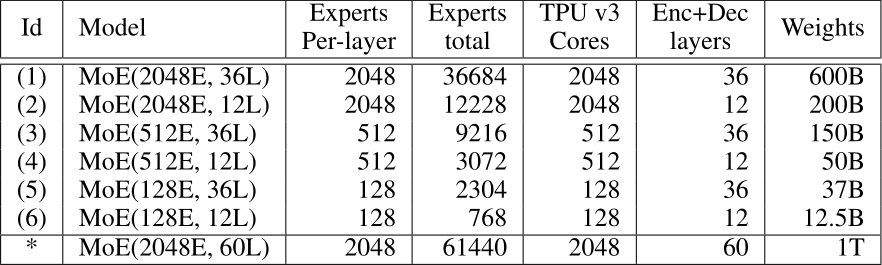
\includegraphics[scale=0.24]{img/gshard_models.png}
        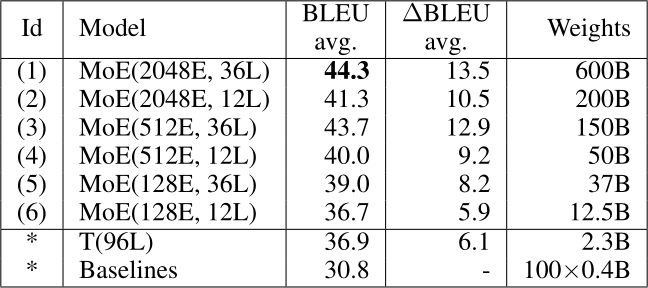
\includegraphics[scale=0.24]{img/gshard_score.png}
        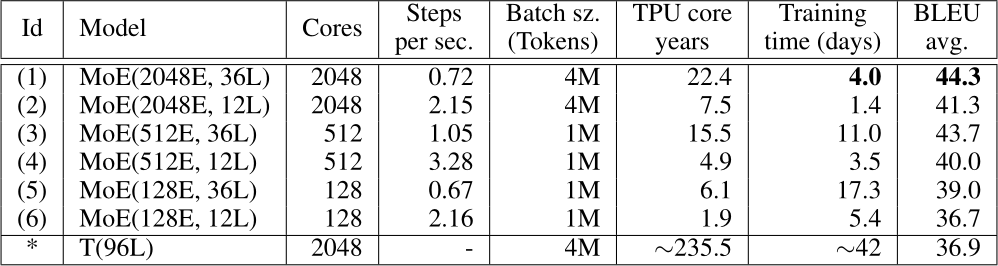
\includegraphics[scale=0.21]{img/gshard_score_2.png}
    \end{center}
\end{frame}



% Switch Transformers
\section{Switch Transformers}
\begin{frame}
    \frametitle{Switch Transformers \cite{switch_transformer}}
    \begin{itemize}
        \item January 2021, Google - code available (Mesh TensorFlow)
        \item Transformer Encoder with MoE (\textbf{Mixture-of-Experts}) layers
        \item \textbf{7x} increases in pre-training speed (compared to T5 model)
        \item scale up to \textbf{trillion parameter} models on C4 (Colossal Clean Crawled Corpus - 180B tokens) dataset
    \end{itemize}
\end{frame}

\begin{frame}
    \frametitle{Architecture}
    \begin{center}
        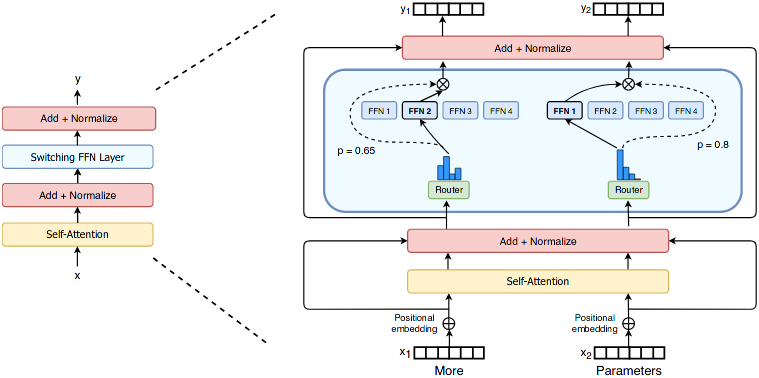
\includegraphics[scale=0.42]{img/switch_transformers_architecture.png}
    \end{center}
\end{frame}

\begin{frame}
    \frametitle{Improved training and fine-tuning techniques}
    \begin{itemize}
        \item \textbf{selective precision with large sparse models} - selective casting (cast the local routing operations to float32 - broadcasting bfloat16 then cast to float32)
    \end{itemize}
    \begin{center}
        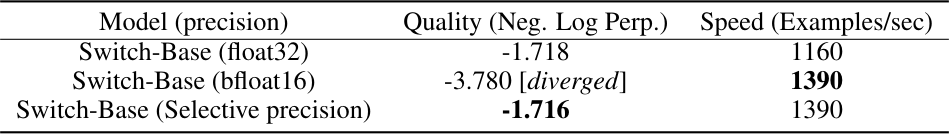
\includegraphics[scale=0.33]{img/switch_transformers_precision.png}
    \end{center}
\end{frame}

\begin{frame}
    \frametitle{Improved training and fine-tuning techniques}
    \begin{itemize}
        \item \textbf{smaller parameter initialization for stability} - use truncated normal distribution and reduce the default initialization scale factor
    \end{itemize}
    \begin{center}
        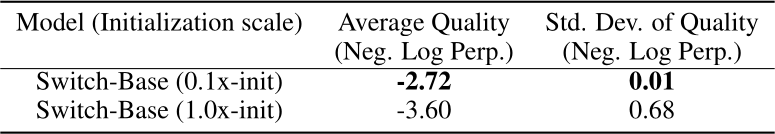
\includegraphics[scale=0.40]{img/switch_transformers_initialization.png}
    \end{center}
\end{frame}

\begin{frame}
    \frametitle{Improved training and fine-tuning techniques}
    \begin{itemize}
        \item \textbf{regularizing large sparse models} - increase the dropout inside the experts (expert dropout) during fine-tuning (bigger models can lead to more severe overfitting on smaller downstream tasks)
    \end{itemize}
    \begin{center}
        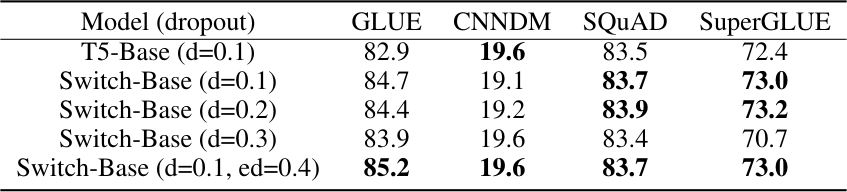
\includegraphics[scale=0.37]{img/switch_transformers_dropout.png}
    \end{center}
\end{frame}

\begin{frame}
    \frametitle{Pre-training on C4 dataset}
    \begin{itemize}
    	\item \scriptsize{128 experts, 100k steps only}
    \end{itemize}
    \begin{center}
        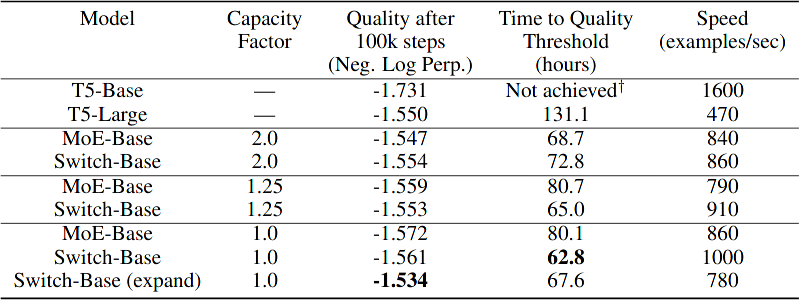
\includegraphics[scale=0.4]{img/switch_transformers_benchmark.png}
        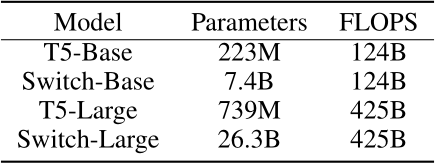
\includegraphics[scale=0.345]{img/switch_transformers_flops.png}
    \end{center}
\end{frame}

\begin{frame}
    \frametitle{Speed up pre-training (with fixed FLOPS per token)}
    \begin{center}
        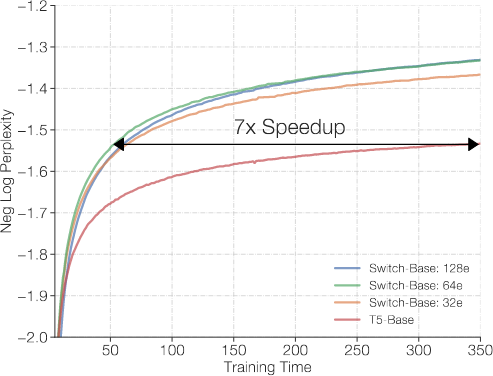
\includegraphics[scale=0.35]{img/switch_transformers_speedup.png}
    \end{center}
    \begin{itemize}
        \item \textbf{Switch-Base 64} expert model achieves the same performance of the \textbf{T5-Base} model at step 60k at step 450k, which is a \textbf{7.5x} speedup in terms of step time
    \end{itemize}
\end{frame}

\begin{frame}
    \frametitle{Speed up pre-training}
    \begin{center}
        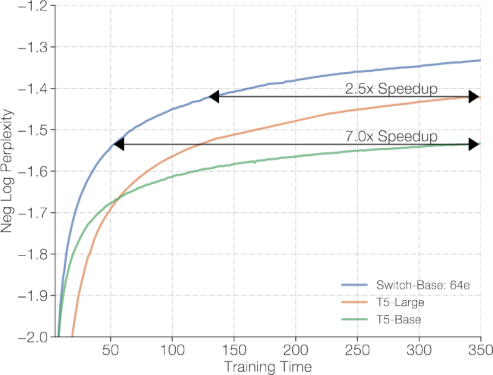
\includegraphics[scale=0.36]{img/switch_transformers_speedup_2.png}
        \begin{itemize}
            \item \textbf{T5-Large} applying \textbf{3.5x} more FLOPs per token
            \item \textbf{Switch-Base} is still more sample efficient and yields a \textbf{2.5x} speedup
        \end{itemize}
    \end{center}
\end{frame}

\begin{frame}
    \frametitle{Fine-tuning results (validation set)}
    \begin{center}
        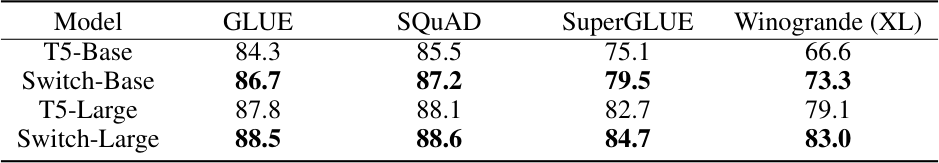
\includegraphics[scale=0.34]{img/switch_transformers_glue.png}
        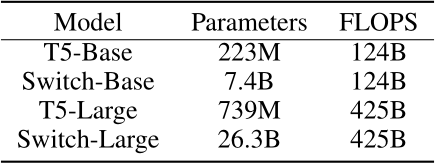
\includegraphics[scale=0.35]{img/switch_transformers_flops.png}
        \begin{itemize}
            \item \textbf{T5} and \textbf{Switch} models were pre-trained on a C4 dataset
        \end{itemize}
    \end{center}
\end{frame}

\begin{frame}
    \frametitle{Distillation (base on DistilBERT - Hugging Face)}
    \begin{center}
        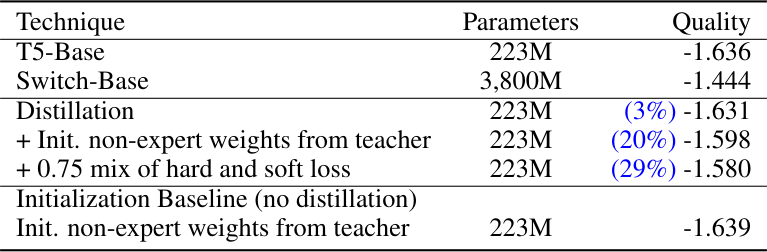
\includegraphics[scale=0.34]{img/switch_transformers_distilled.png}
        \begin{itemize}
            \item pre-training distillation
            \item initialize the dense model with the non-expert weights
            \item use a mixture of 0.25 for the teacher probabilities and 0.75 for the ground truth label
            \item no improvement of \textbf{T5-Base} initialized with the expert weights
        \end{itemize}
    \end{center}
\end{frame}

\begin{frame}
    \frametitle{Distillation compression rates}
    \begin{center}
        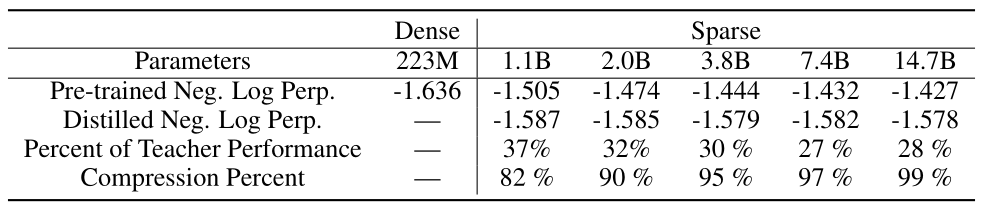
\includegraphics[scale=0.33]{img/switch_transformers_distilled_all.png}
        \begin{itemize}
            \item \textbf{preserve 37\% of the quality} gain of the 1.1B parameter model while \textbf{compressing 82\%}
            \item the extreme, preserve 28\% of the quality gain of the 14.7B parameter model while compressing 99\%
        \end{itemize}
    \end{center}
\end{frame}

\begin{frame}
    \frametitle{Distilling a fine-tuned mode}
    \begin{center}
        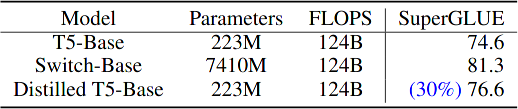
\includegraphics[scale=0.45]{img/switch_transformers_distilled_final.png}
        \begin{itemize}
        	\item fine-tuned sparse model into a dense model
            \item on smaller datasets large sparse model can be an effective teacher for distillation
            \item achieve 30\% of the teacher’s performance on a 97\% compressed model
        \end{itemize}
    \end{center}
\end{frame}

\begin{frame}
    \frametitle{Multilingual pre-training on 101 languages (mT5)}
    \begin{center}
        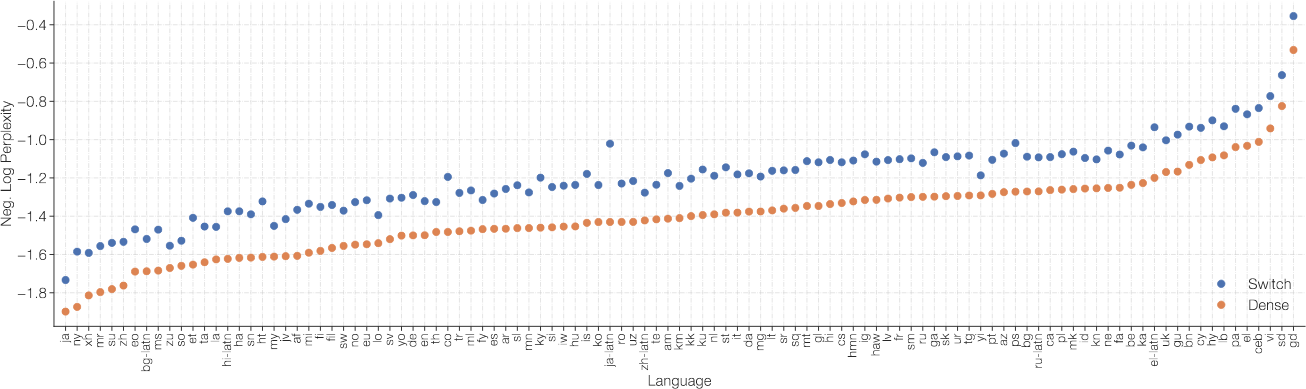
\includegraphics[scale=0.25]{img/switch_transformers_multilingual_pretraining.png}
        \begin{itemize}
            \item pre-train on the multilingual variant of the Common Crawl dataset (mC4)
            \item \textbf{mSwitch-Base} is 5x faster than \textbf{mT5-Base} (4x on 91\% of languages)
        \end{itemize}
    \end{center}
\end{frame}

\begin{frame}
    \frametitle{How the model weights/data are split?}
    \begin{center}
        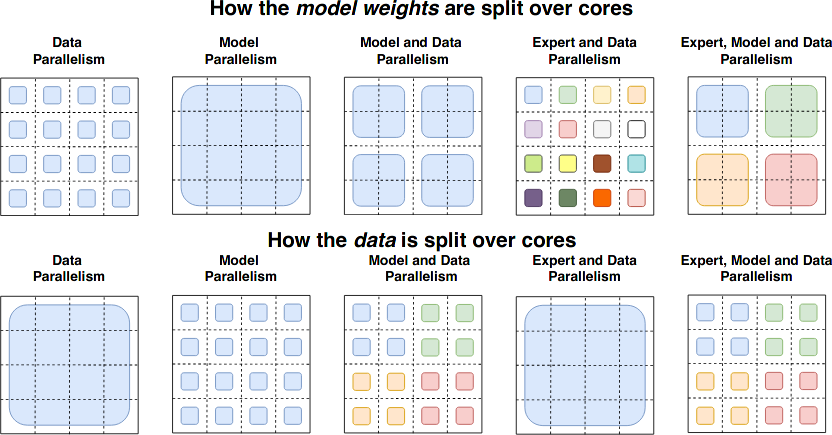
\includegraphics[scale=0.39]{img/switch_transformers_model_data_distribution.png}
    \end{center}
\end{frame}

\begin{frame}
    \frametitle{Switch for Attention}
    \begin{center}
        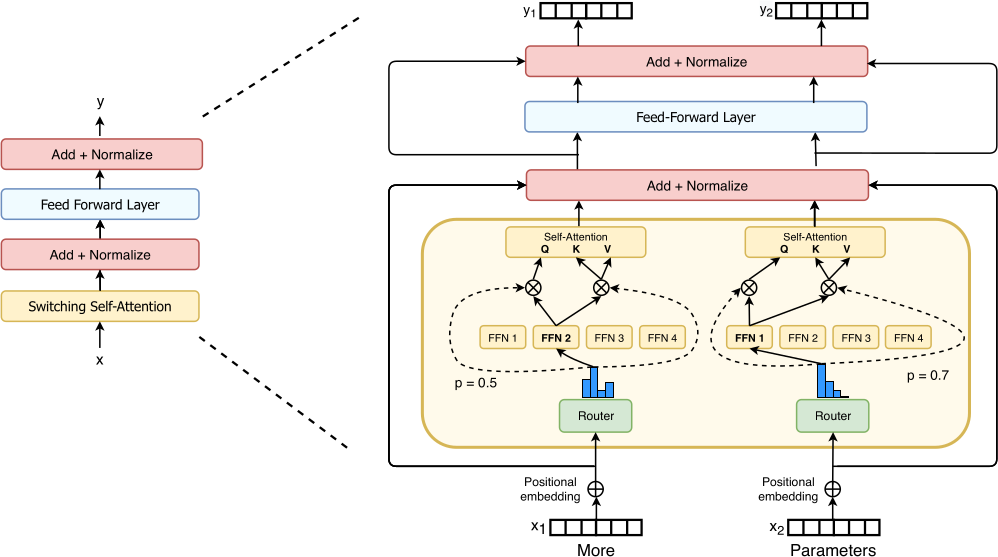
\includegraphics[scale=0.3]{img/switch_transformers_attention.png}
    \end{center}
\end{frame}

\begin{frame}
    \frametitle{Switch for Attention}
    \begin{center}
        \begin{itemize}
            \item add \textbf{Switch layers} into the \textbf{Transformer Self-Attention layers}
            \item replace the \textbf{trainable weight matrices that produce the queries, keys and values} with \textbf{Switch layers} (one set of weights produces the query and the other set of unique weights produces the shared keys and values)
            \item found this to be \textbf{more unstable} when used with low precision number formats, and thus leave it for future work
        \end{itemize}
        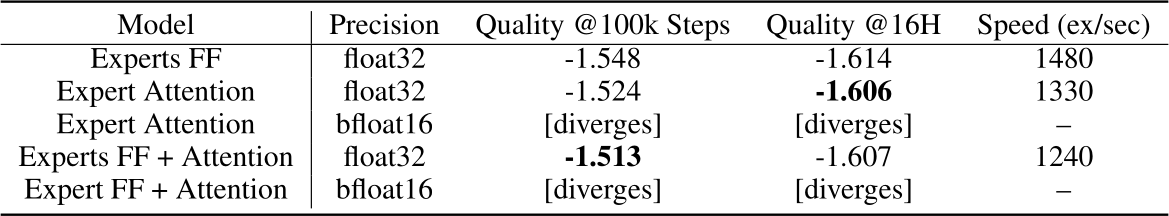
\includegraphics[scale=0.28]{img/switch_transformers_attention_result.png}
    \end{center}
\end{frame}

\begin{frame}
    \frametitle{Switch Transformer in lower compute regimes (recommend one expert per core)}
    \begin{center}
        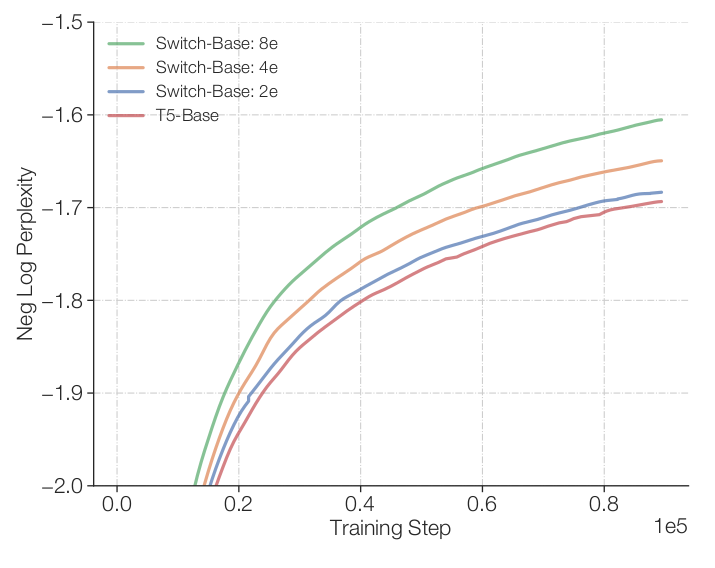
\includegraphics[scale=0.35]{img/switch_transformers_low_resources.png}
    \end{center}
\end{frame}



% Feedback Transformers
\section{Feedback Transformers}
\begin{frame}
    \frametitle{Feedback Transformers \cite{feedback_transformer}}
    \begin{itemize}
        \item 2020, Facebook - no code available
        \item Transformer Decoder (autoregressive model)
        \item Feedback memory (exposes all previous representations to all future representations) - recursive computation
        \item tested on language modeling, machine translation and reinforcement learning
        \item Feedback Transformer is not much slower compared to the standard Transformer
    \end{itemize}
\end{frame}

\begin{frame}
    \frametitle{Feedback Transformer}
    \begin{itemize}
        \item makes \textbf{all previous hidden representations accessible} to the computation of a representation at any depth
        \item merges \textbf{the hidden states from all layers into a single
vector} for every time step and stores them in a memory (every previously computed representation is accessible)
    \end{itemize}
    \begin{center}
        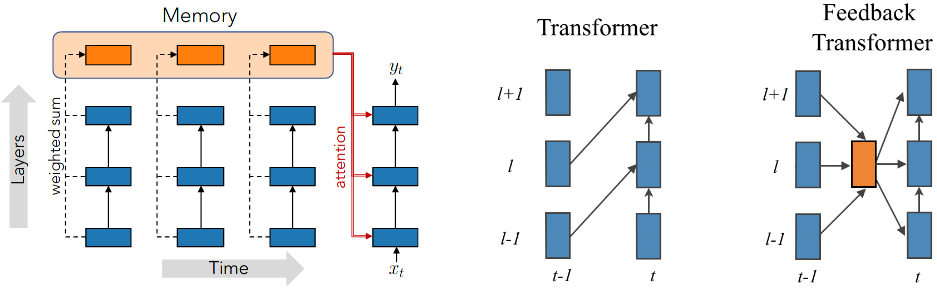
\includegraphics[scale=0.34]{img/feedback_transformer_architecture.png}
    \end{center}
\end{frame}

\begin{frame}
    \frametitle{Feedback memory}
    \begin{itemize}
        \item uses less memory because  \textbf{all the layers share a single Feedback memory}, thus \textbf{reducing the memory} size by L times (L is the number of layers)
        \item \textbf{uses less computation} because \textbf{share the key} and \textbf{value projections} during attention computation, which increases the speed of the attention
        \item GPU memory usage is reduced due to the \textbf{memory sharing} — the
overall model is 2x smaller
    \end{itemize}
\end{frame}

\begin{frame}
    \frametitle{Feedback Transformer Attention}
    \begin{center}
        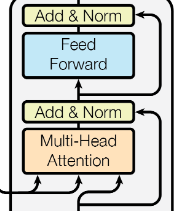
\includegraphics[scale=1.2]{img/cross_attention.png}

        \begin{tabular}{ l r }
        \scriptsize{\textbf{Transformer Attention} = Attn(Q, VK)} \\
        $ z_{t}^{l} = $ Attn $( x_{t}^{l}, \{ x_{t - \tau}^{l}, ...,  x_{t - 1}^{l} \} )$ & $ x_{t}^{l + 1} = $ FF $( z_{t}^{l} )$ \\
        \hline
        \scriptsize{\textbf{Feedback Transformer Attention}} \\
        $ z_{t}^{l} = $ Attn $( x_{t}^{l}, \{ \textbf{m}_{t - \tau}^{l}, ..., \textbf{m}_{t - 1}^{l} \} )$ & $ x_{t}^{l + 1} = $ FF $( z_{t}^{l} )$ \\
        $m_t = \sum_{l=0}^{L} $ Softmax $(w^l) x_t^l$
        \end{tabular}
    \end{center}
    \begin{itemize}
        \item \scriptsize{sharing the \textbf{key} and \textbf{value} projections $W_k^l$ and $W_v^l$ across all layers:

        $ k_l^t = k_t = W_k m_t$ and $v_t^l = v_t = W_v m_t $}
    \end{itemize}
    \begin{center}
        \scriptsize{$l$ - layer of Transformer, $ x_{t - \tau}^{l}, ...,  x_{t - 1}^{l} $ - past context/vectors, $t$ - sequence length}, $\textbf{m}$ - memory vectors, $w^l$ - learnable scalar parameters (flexibility in averaging/selecting layers)
    \end{center}
\end{frame}

\begin{frame}
    \frametitle{Score - accuracy on toy tasks}
    \begin{center}
        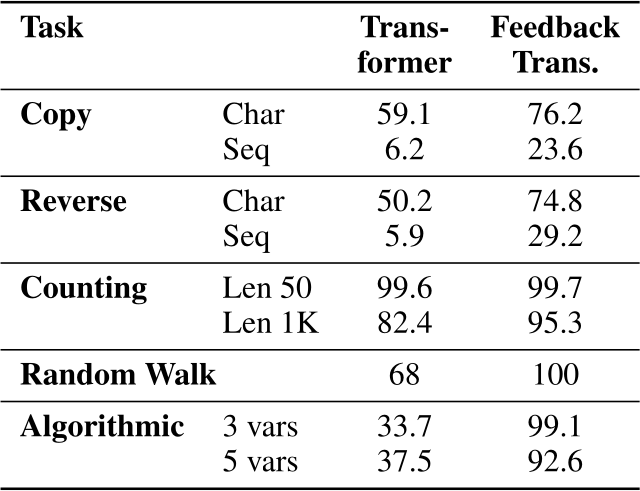
\includegraphics[scale=0.18]{img/feedback_transformer_copy_reverse.png}
    \end{center}
    \begin{itemize}
        \item \scriptsize{\textbf{Copy and Reverse} - models read the input and then either copy or reverse}
        \item \textbf{Counting} - models have a sequence of $A$ in a row, and must output the corresponding quantity of the letter $B$
        \item \textbf{Random Walk} - random walk in a small grid where the goal is calculate the current position
        \item \textbf{Algorithmic task} - tracking and updating value of variables in code execution (needs keep track of all variable values and update them if necessary)
    \end{itemize}
\end{frame}

\begin{frame}
    \frametitle{Score - Machine Translation on WMT14 En-De}
    \begin{center}
        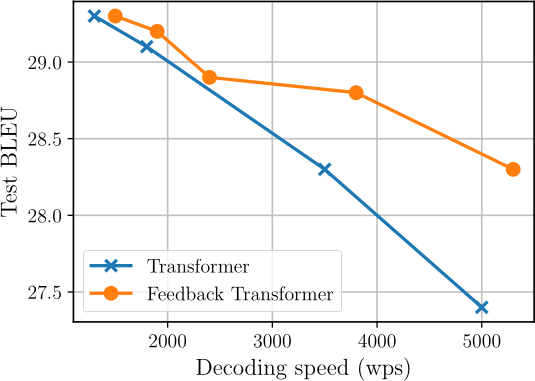
\includegraphics[scale=0.3]{img/feedback_transformer_wmt_decoding.png}
    \end{center}
    \begin{itemize}
        \item model \textbf{shallower} only — layers are removed from a Transformer decoder
        \item the \textbf{1-layer Transformer} model can only reach \textbf{27.3}, the Feedback Transformer has \textbf{28.3} BLEU
    \end{itemize}
\end{frame}

\begin{frame}
    \frametitle{Compare to other architectures - WMT En-De}
    \begin{center}
        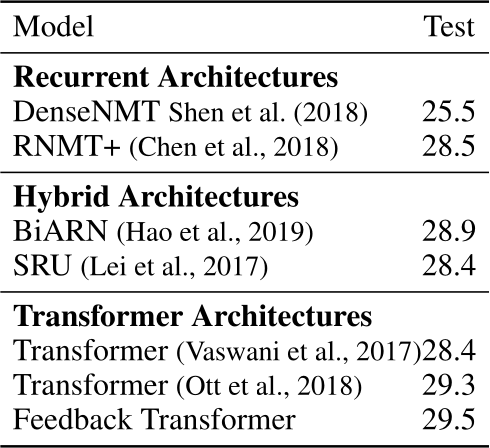
\includegraphics[scale=0.3]{img/feedback_transformer_compare_architectures.png}
    \end{center}
\end{frame}

\begin{frame}
    \frametitle{Compare memorization strategy}
    \begin{itemize}
        \item Feedback Transformer = all
    \end{itemize}
    \begin{center}
        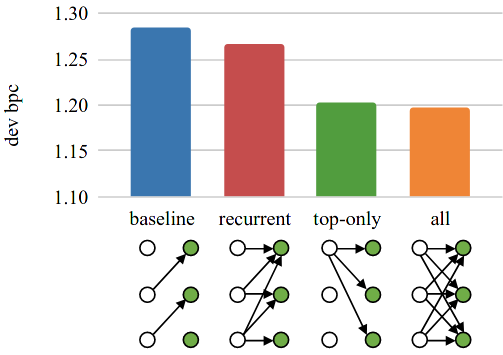
\includegraphics[scale=0.42]{img/feedback_transformer_compare_memory.png}
    \end{center}
\end{frame}

\begin{frame}
    \frametitle{Ablation studies}
    \begin{center}
        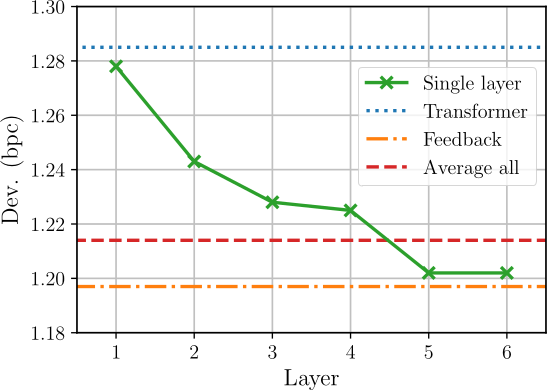
\includegraphics[scale=0.35]{img/feedback_transformer_compare_ablation.png}
    \end{center}
    \begin{itemize}
        \item \footnotesize{\textbf{Feedback Transformers} - weighted sum of all layers}
        \item \textbf{Single layer} - manually select one of the layers as the memory
        \item \textbf{Average all} - averaging all layers together
    \end{itemize}
\end{frame}

\begin{frame}
    \frametitle{Score - WikiText-103}
    \begin{center}
        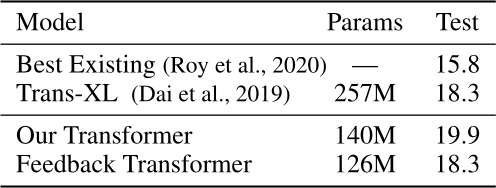
\includegraphics[scale=0.3]{img/feedback_transformer_wikitext103.png}
    \end{center}
    \begin{itemize}
        \item Best - \textbf{Routing Transformer} (sparse attention patterns, 2020)
        \item Feedback Transformer train \textbf{3.5 days}, compared to the Transformer which takes \textbf{1.2 days}
        \item train small Feedback Transformer - \textbf{half the size} of Transformer-XL (match the performance of Transformer-XL)
        \item \textbf{the same size} as standard Transformer has \textbf{worse performance} (19.9 PPL rather than 18.3)
    \end{itemize}
\end{frame}

\begin{frame}
    \frametitle{Score - Enwiki8}
    \begin{center}
        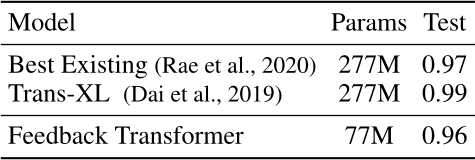
\includegraphics[scale=0.3]{img/feedback_transformer_enwiki8.png}
    \end{center}
    \begin{itemize}
        \item \textbf{character-level} language modeling - containing 100M unprocessed bytes from Wikipedia
        \item train a relatively small 12-layer model, that is \textbf{one third} of the size of the Transformer-XL baseline
    \end{itemize}
\end{frame}

\begin{frame}
    \frametitle{Training and Inference Speed}
    \begin{center}
        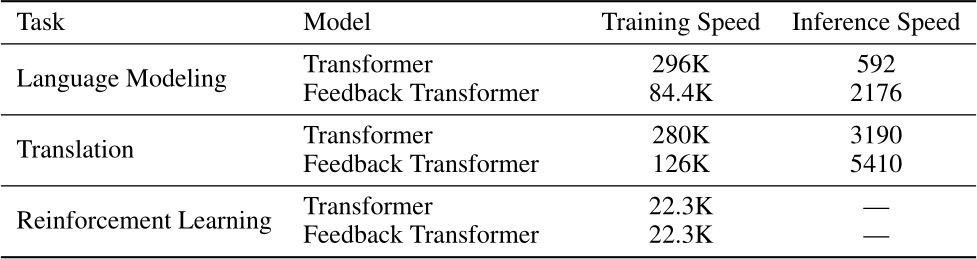
\includegraphics[scale=0.34]{img/feedback_transformer_time.png}
    \end{center}
\end{frame}



% GPT-Neo
\section{GPT-Neo}
\begin{frame}
    \frametitle{GPT-Neo}
    \begin{itemize}
        \item July 2020, EleutherAI - Tensorflow-mesh
        \item \textbf{replication of OpenAI} massive 175B parameter language model (GPT-3) and open source it to the public
        \item the largest model trained for a single step so far has been 200B parameters
        \item GPT-2 size models trained
        \item several experimental architectures implemented (e.g. Linear attention,  Mixture of Experts, Masked Language Modeling)
    \end{itemize}
\end{frame}

% References
\section{References}
\begin{frame}[allowframebreaks,t]
    \tiny
    \frametitle{References}
    \bibliographystyle{ieeetr}
    \bibliography{switch_transformer}
    %\nocite{*}
\end{frame}

\end{document}
